\chapter{Revisão da literatura}

\section{Preliminar}

A crescente pesquisa por análise de sentimentos e \textit{text mining} tende a corroborar, de forma geral, para um melhor entendimento do que acontece no cenário mundial econômico, por meio de \textit{proxys} que por muitas vezes não podem ser captadas senão de forma computacional. Compreender melhor a demanda por alguma coisa torna-se mais fácil, no quesito em que é possível automatizar resoluções de problemas econômicos e não econômicos. Como um próprio exemplo disso, podemos nos fazer valer da própria busca pelo termo \textit{sentiment analysis}. A Figura \ref{fig:google} apresenta a evolução da busca pelo termo \textit{sentiment analysis}, desde 2004 até o mês de outubro de 2019 -- A busca foi realizada no dia primeiro de novembro de 2019, com os seguintes parâmetros: 1 - termo de pesquisa: sentiment analysis; 2 - foi aplicado um período de busca de 2004 até o mês de outubro de 2019; Para todo o mundo, todas as categorias, e pesquisa na web. No volume de busca, 100 representa o máximo volume como referência. 

\begin{figure}[!h]
    \centering
    \caption{Evolução da busca pelo termo \textit{sentiment analysis}, de janeiro de 2004 até outubro de 2019}
    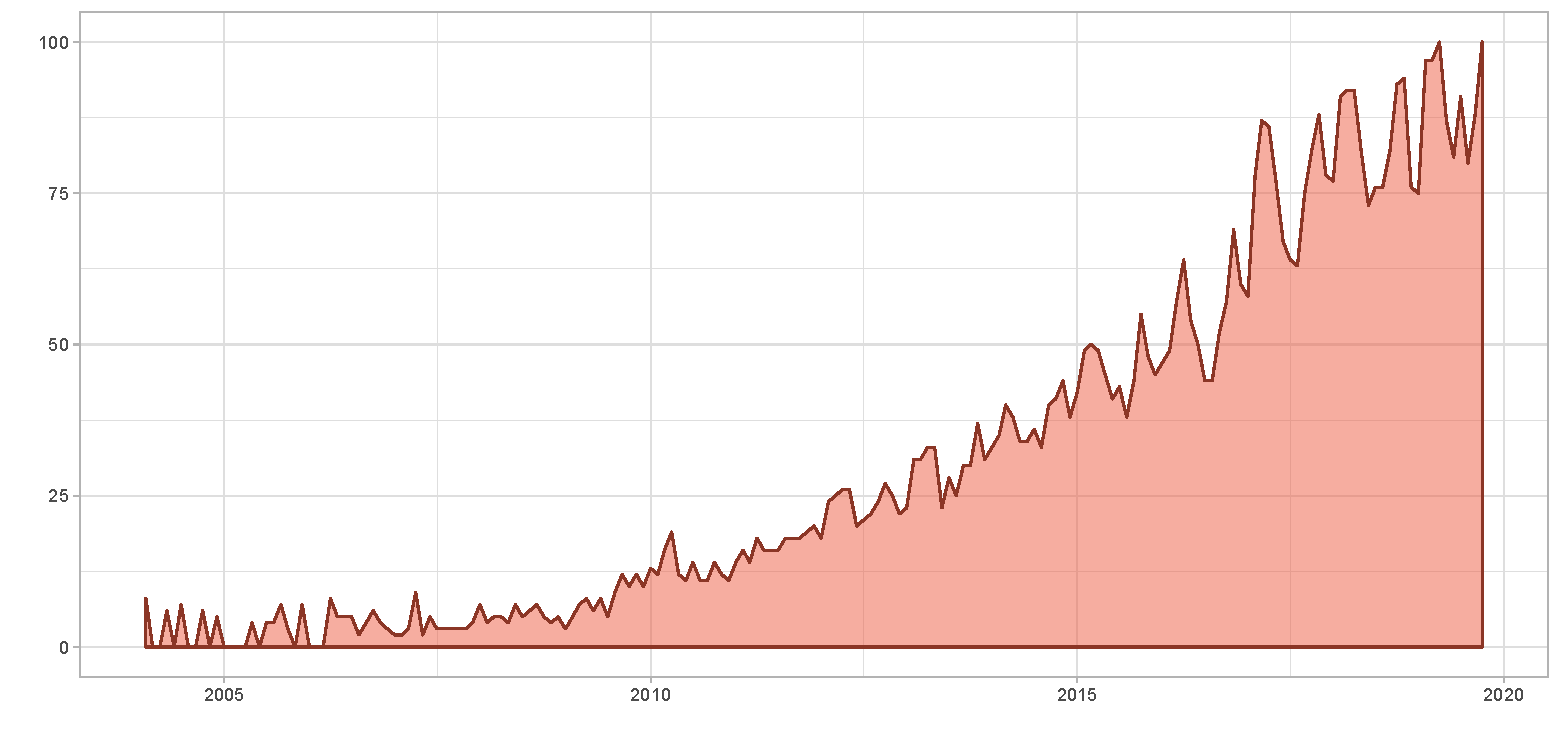
\includegraphics[width=\textwidth]{capitulos/figures/google.pdf}
    \fonte{Google trends. Elaboração própria.}
    \label{fig:google}
\end{figure}

Ainda, acrescenta-se, mesmo que atualmente o volume de buscas por esse termo seja quase insignificante para o Brasil (cerca de 4), países como a Índia ou a China apresentam volumes de buscas muito maiores: 81 e 22, respectivamente. A Índia é o pais que mais busca por esse termo. Tal qual, pode ser uma relação direta na crescente potencialidade tecnológica e de pesquisa deste país. 

\section{Mineração Textual}

Processamento de linguagem natural, conhecido também como \textit{Text Minning}, é um conjunto de procedimentos que utiliza ferramentas computacionais e técnicas estatísticas que permitem quantificar textos. Este processo de quantificação permite intuir algum significado textual -- indubitavelmente, por meio de um computador a análise e organização dos significados textuais podem ser feitas de formam muito mais precisa e automática do que de forma manual. O \textit{text mining}, ainda, possibilita a extração de \textit{significados} de textos, que podem ser difíceis de se identificar quando analisados sem o auxílio de um computador -- nos permite detectar padrões pouco prováveis ante às perspectivas humanas.

Mesmo quando muito usada em outros campos científicos, como ciências políticas e marketing, a técnica de \textit{text minning} ainda é pouco utilizada nas ciências econômicas como enuncia \citeonline{bholat2015text}

\begin{citacao}``Primeiro, pode não ser óbvio que o texto possa ser descrito e analisado como dados quantitativos. Como resultado, provavelmente existe uma falta de familiaridade nos bancos centrais com as ferramentas e técnicas estatísticas que tornam isso possível. Segundo, mesmo que os banqueiros centrais tenham ouvido falar em mineração de texto, eles já têm acesso a outros dados quantitativos prontamente disponíveis. A oportunidade e outros tipos de custos de transformar textos em dados quantitativos e aprender novas ferramentas e técnicas para analisar esses dados podem ser vistos como superando os benefícios esperados.
\footnote{First, it may not be obvious that text can be described and analysed as quantitative data. As a result, there is probably a lack of familiarity in central banks with the tools and statistical techniques that make this possible. Second, even if central bankers have heard of text mining, they already have access to other readily available quantitative data. The opportunity and other types of costs from transforming texts into quantitative data, and learning new tools and techniques to analyse these data, may be viewed as outweighing the expected benefits. \cite[p.1]{bholat2015text}}'' \cite[p.1]{bholat2015text}
\end{citacao}

Assim, a inserção do \textit{text mining} no campo da ciência econômica se apresenta de forma tardia, devido a obstáculos computacionais e por vezes desconfiança por parte dos agentes econômicos acostumados com informações quantitativas tradicionais. Uma análise a partir destes pode, ainda mais, incluir aspectos não convencionais em modelos micro e macroeconômicos, como possíveis \textit{proxys} de conjuntura política, interesses populacionais ou mesmo opiniões públicas. É notável, então, que a utilização de técnicas de \textit{text mining} poderia ser utilizada de maneira extremamente proveitosa por, por exemplo, bancos centrais. Isso é, extrair informações de formas não usuais de fontes que permitam, de alguma forma, avaliar estabilidade monetária e financeira de maneira quantitativa. Ou seja, a partir de notícias, jornais, artigos científicos, relatos de inteligência de mercado, ou mesmo relatórios empresariais, afim de quantificar estes dados para uma melhor obtenção da situação conjuntural vigente. 

A análise de um documento, ou um conjunto de documentos (tecnicamente chamado de \textit{corpus}) se daria, por exemplo, a partir de boletins informacionais de órgãos de pesquisa (vide por exemplo uma carta de conjuntura do Ipea - Instituto de Pesquisa Econômica Aplicada) ou mesmo atas de instituições financeiras.

Mesmo que ainda não seja uma técnica usual de análise, bancos centrais já se fazem valer de benefícios do \textit{text mining} diariamente. Uma busca online por determinados termos econômicos, dependendo da forma como é feita, ou mesmo proteção contra \textit{cyber-attacks} ou busca por uma base de dados de citações, no âmbito acadêmico, são exemplos usuais da funcionalidade do \textit{text mining} \cite{bholat2015text}.

\section{Análise de Sentimentos}

Em um recente artigo publicado pelo Banco da Inglaterra, \citeonline{bholat2015text},  é relatado os interesses dos bancos centrais e como estes, por meio textuais, não são devidamente aproveitados. Um exemplo de aplicação em relação a estes volumes de dados é a própria pesquisa realizada na internet, em termos econômicos ou mesmo em relação ao volume de buscas. Ainda podemos citar a correlação entre Jobseeker’s Allowance (JSA) e a taxa oficial de desemprego no Reino Unido, como mostra \citeonline{mclaren2011using}:

\begin{citacao}``É notável que os 'empregos', que provavelmente foram pesquisados por quem está dentro e fora do emprego, não aumentaram muito durante a recessão. As pesquisas por "desempregados" aumentaram acentuadamente durante a recessão. O termo "JSA" (sigla para Subsídio de Desemprego) foi escolhido porque seus movimentos melhor se correlacionaram com os dos dados oficiais. Também é provável que seja usado por aqueles que pensam que podem em breve ficar desempregados e, portanto, buscam mais informações sobre benefícios de desemprego.\footnote{It is notable that ‘jobs’, which is likely to have been searched for by both those in and out of employment, did not increase much during the recession.  Searches for ‘unemployed’ rose markedly during the recession.  The term ‘JSA’ (acronym for Jobseeker’s Allowance) was chosen because its movementsbest correlated with those in the official data.  It is also a termlikely to be used by those who think they may soon become unemployed and so search for more information on unemployment benefit. \cite[p.136]{mclaren2011using}}'' \cite[p.136]{mclaren2011using}
\end{citacao}

Faz sentido uma busca na internet por ``emprego'' quando a pessoa está desempregada, bem como por ``auxílio desemprego'' (Jobseeker’s Allowance). No mesmo artigo, os autores vão além: é possível identificar, ainda, uma correlação entre ``inflação imobiliária'' e ``agentes imobiliários''. Assim, a partir de expressões como ``preços de casas''; ``comprar imóvel''; e ``vender imóvel'' é possível obter uma \textit{proxy} para a demanda por moradia:

\begin{citacao}``Para o mercado imobiliário, segue-se uma abordagem semelhante à adotada acima para o mercado de trabalho. Uma proporção significativa de pesquisas relacionadas a habitação é para sites de empresas específicas. No entanto, essas pesquisas variam ao longo do tempo, dependendo da popularidade de cada site. Portanto, uma ampla variedade de termos de pesquisa genérica é considerada (incluindo "preços de casas", "casa de compra", "casa de venda", "hipoteca" e "agentes imobiliários"). Os termos de pesquisa 'comprar casa' e 'vender casa' foram inicialmente considerados, pois capturariam a demanda e a oferta de casas.\footnote{For the housing market a similar approach is followed to thattaken above for the labour market.  A significant proportion ofhousing-related searches are for specific companies’ websites.However, these searches vary over time depending on thepopularity of each website.  So a wide range of more genericsearch terms are considered (including ‘house prices’, ‘buyhouse’, ‘sell house’, ‘mortgage’ and ‘estate agents’).  The searchterms ‘buy house’ and ‘sell house’ were initially considered,since they would capture the demand for and supply of houses. \cite[p.137]{mclaren2011using}}'' \cite[p.137]{mclaren2011using}
\end{citacao}

Em ambos os casos, os autores obtiveram exito em suas pesquisas, o artigo ``Using internet search data as economic indicators'' \cite[p.136]{mclaren2011using}, publicado também pelo Banco da Inglaterra, apresenta resultados econométricos significativos frente a regressões utilizando variáveis reais regredidas em variáveis obtidas por meio de volume de buscas online. Isso é, seja em relação à taxa de desemprego como em relação à inflação imobiliária, ambas as séries puderam ser explicadas por meio das séries dos volumes de pesquisa online -- Nos exemplos citados no texto, o mecanismo de busca utilizado foi o \textit{google trends}.

Outra maneira de se aproveitar algorítimos e volumes de buscas online é levar em consideração medidas de risco e incerteza no âmbito econômico e financeiro dado um determinado momento. Uma recente contribuição nessa direção foi apresentada por \citeonline{nyman2018news}: é proposta uma teoria sobre ``hipótese financeira emocional'', a qual sustenta que ``os indivíduos se convencem a assumir posições nos mercados financeiros, criando narrativas sobre os possíveis resultados de suas ações''\footnote{``individuals gain conviction to take positions in financial markets by creating narratives about the possible outcomes of their actions'' \cite{nyman2018news, bholat2015text}}. Os autores correlacionam emoções de ``exitação'' com ganhos financeiros e ``ansiedade'' com possíveis perdas. Essas narrativas, entretanto, não são compostas de simples textos, e sim de interações sociais entre agentes. As hipóteses foram testadas a partir de três textos fundamentais: the Bank’s daily market commentary (2000-2010), broker research reports (2010-2013) and the Reuters’ News Archive (1996-2014). A partir disto, os autores propõe um índice de medida de sentimento textual:

$$SI_t=\frac{N_e - N_a}{N_t}$$ 

\noindent
onde $N_e$ e $N_a$ representam o número de palavras correlacionadas com os estados de, respectivamente, excitação e ansiedade. $N_t$ denota o número total de palavras do documento. O sinal do índice nos fornece um indicativo do que acontece no mercado: sendo esse positivo é simbolizado crescimento financeiro; caso negativo, uma retração no mercado financeiro -- respectivamente \textit{bullish} e \textit{bearish}.
%caso positivo, há o chamado \textit{bullish}\footnote{No mercado financeiro, \textit{bullish} representa o ataque de um touro. Isso é, atacando de baixo para cima -- simbolizando o crescimento financeiro} - isso é, quando o mercado está em ascensão; caso contrário (sinal negativo), determina-se um momento de \textit{bearish}\footnote{No mercado financeiro, \textit{bearish} representa o ataque de um Urso. Isso é, atacando de cima para baixo -- simbolizando uma queda financeira}
O índice, então, é comparado com outros eventos históricos e outros indicadores financeiros \cite{bholat2015text}. 

Uma vez que a incerteza econômica é medida, esta poderia ser utilizada como uma variável explicativa em modelos de bancos centrais - essa torna-se, então, um possível indicador quanto às orientações de política monetária de bancos centrais.

A análise de sentimentos pode ser definida como o resultado de uma sequência hierarquizada de processos de ``classificação''. Por sua vez, a classificação é entendida como uma função, ou domínio, em um conjunto de entidades e imagens em um conjunto binário: positivo, negativo. Indo além, existem três principais níveis de classificação em análise de sentimento: documento, aspecto e sentença.

\begin{citacao}``
Em documentos o objetivo é classificar a opinião do documento como expressando um sentimento ou opinião positiva ou negativa. É considerado o documento em sua totalidade como uma unidade de informação (falando sobre um tópico). Com
relação às sentenças, o objetivo é classificar o sentimento expresso em cada sentença. O primeiro passo é identificar se a sentença é subjetiva ou objetiva. Se a sentença é subjetiva a análise determinará se a sentença expressa opiniões positivas ou negativas. Já em nível de aspecto, o alvo é classificar o sentimento com relação as aspectos específicos das entidades a partir da identificação das entidades e seus aspectos dada a possibilidade de existir diferentes opiniões sobre aspectos distintos da mesma entidade (como em: A qualidade da chamada do telefone não é boa, mas a bateria dura muito tempo). '' \cite[p.12]{costa2016ensaios}
\end{citacao}

Em geral, pode-se classificar algorítimos de análise de sentimentos de duas formas: baseados em \textit{machine learning}, sendo possível dividir esses algorítimos em forma de aprendizado supervisionado e aprendizado não supervisionado; a outra forma é trabalhar por meio de dicionários (\textit{léxicos}). Como exemplo, podemos citar o dicionário \texttt{qdap} contido no pacote de mesmo nome do R implementado por \citeonline{qdapdict} que pode determinar, segundo seus critérios de análise, se uma palavra pode ser classificada como positiva ou negativa.

Para exemplificarmos a utilização de um dicionário léxico, um trabalho recente de \citeonline{costa2016ensaios}, apresenta uma análise de sentimentos para as atas do Comitê de Política Monetária para o período de 2000 à 2016. No estudo, um \textit{corpus} é composto por 157 atas e analisado e, por meio deste, um índice é proposto, onde $I_t$ é o índice de sentimento:
\begin{align} \label{indicecosta}
    I_t = \frac{NP_t - NN_t}{N} \quad ,
\end{align}


\noindent
para cada ata divulgada em $t$, $NP_t$ é a quantidade de palavras ``positivas'', $NN_t$ a quantidade de palavras ``negativas'', e $N$ a quantidade de palavras na ata \cite[p.13]{costa2016ensaios}.

Os autores chegam a conclusão, finalmente, de uma correlação entre determinadas variáveis macroeconômicas (taxa de juros Selic, IPCA, IPCA Meta) e o índice para tomada de decisão da autoridade monetária. A correlação se apresenta de maneira mais forte no que diz respeito ao comportamento de longo prazo dessas variáveis. Em períodos de alta de inflação há uma diminuição do \textit{score} do índice de sentimentos, o que representa uma maior cautela na expectativa econômica representada pela maior quantidade de palavras ``negativas'' utilizadas nas atas divulgadas no período analisado. Comportamento análago ocorre quando se compara o \textit{score} do índice com a taxa de juros Selic.

\section{Aplicações Econométricas}

Formuladores de políticas econômicas (\textit{policy makers}) e aqueles que participam do mercado confiam amplamente em uma variedade de modelos que incorporam o que é chamado de informação branda. Ao contrário de informações complexas, que incluem variáveis objetivas e diretamente quantificáveis (como produção e taxa de desemprego), informações brandas influem medidas subjetivas relativas a atitudes em relação às condições econômicas atuais e futuras. Há, assim, uma ampla variedade de variáveis flexíveis disponíveis, mas sem dúvida as mais amplamente levadas em consideração  são as medidas relativas às confianças de mercado e sentimento do consumidor \cite{shapiro2018measuring}.

No artigo ``Measuring News Sentiment'' de \citeonline{shapiro2018measuring}, mais um índice de sentimentos foi proposto levando em consideração a estimação dos efeitos de positividade em artigos de forma mensal. Isto é, os autores consideram positividades em artigos em jornais de cunho econômico. 

Este índice de sentimento proposto foi utilizado como um exercício de aplicação, relacionando-o com a atividade econômica dos Estados Unidos. Neste exercício, é avaliado se especificamente a positividade do índice surte algum efeito na atividade econômica futura. Para isso foi utilizado o o método de projeção local proposto por \citeonline{jorda2005estimation}, similar a um vetor auto-regressivo (VAR), porém, menos restritivo. De forma geral, este método analisa como um choque do novo índice de sentimentos afeta um dado nível de atividade econômica. O novo choque do índice de sentimentos é construído como um componente da nova série de sentimentos que é ortogonal a atual e a seis defasagens de atividade econômica bem como a seis defasagens de si mesmo. Isso é, para cada previsão num horizonte $h$, uma regressão diferente é estimada para cada valor da atividade econômica calculada ($y_j$) no momento respectivo e defasado do novo índice de sentimentos e de outras quatro medidas econômicas (consumo, produção, taxa de juros real, e inflação) \cite{shapiro2018measuring}.

Feita a estimação, chega-se a conclusão que um choque positivo no índice de sentimentos, afeta positivamente o consumo, bem como na produção, e na taxa de juros real do FED. Houve, entretanto, uma leve redução para o nível de preços. O efeito no nível de preços é transitório, mas os efeitos no consumo, na produção e na taxa real dos fundos são mais duradouros, aumentando gradualmente até 12 meses após o choque, nas palavras de \citeonline{shapiro2018measuring}.


\begin{citacao}
``Estender o horizonte ainda mais [\dots] indica que as respostas de consumo, produção e taxa real atingem um pico entre 12 e 18 meses após o choque, antes de diminuir gradualmente.\footnote{Extending the horizon out further [\dots] indicates that the responses of consumption, output, and the real rate peak between 12 and 18 months after the shock before gradually waning.}'' \cite[p.19-20]{shapiro2018measuring}
\end{citacao}

Isso é, é possível avaliar uma notável melhora nas variáveis macroeconômicas, ainda, após os 12 meses a frente estimados no impulso resposta.

Em outro artigo \citeonline{shapiro2018measuring} tiveram como inspiração um segundo artigo de \citeonline{barsky2012information} -- que apresenta resultados semelhantes, foi verificado que um choque positivo de sentimentos leva a um aumento persistente em consumo, produção, e taxa real de juros; mas resulta em uma queda na inflação. A similaridades dos resultados, assim, fortalece a hipóteses que um possível índice de sentimentos tem medidas similares em impactos macroeconômicos, como por exemplo, o índice de sentimentos do consumidor.

%No artigo ``Measuring News Sentiment'' de \citeonline{shapiro2018measuring}, mais um índice de sentimentos foi proposto levando em consideração a estimação dos efeitos-fixos do mês $\hat{f}_{t(a)}^i$ a partir da seguinte regressão \cite[p.17]{shapiro2018measuring}:

%$$s_a^i = f_{t(a)}^i + f_{p(a),j(a)}^i + \epsilon_a^i \quad ,$$

%\noindent
%onde $s_a^i$ é o \textit{score} de positividade para o artigo $a$, $f_{t(a)}^i$ é a amostra do mês de referência ($t$) para o efeito fixo. Jornais são indexados por $j$ e artigos - independente do tipo, seja este regular ou não - são anexados por $ f_{p(a),j(a)}^i$ 

%Esse novo índice de sentimento proposto foi utilizado como um exercício de aplicação, relacionando-o com a atividade econômica dos Estados Unidos. Foi avaliado se especificamente este novo índice de atividade econômica surte algum impacto na atividade econômica futura. Para isso foi utilizado o o método de projeção local proposto por \citeonline{jorda2005estimation}, similar a um vetor auto-regressivo (VAR), porém, menos restritivo. De forma geral, este método analisa como um choque do novo índice de sentimentos afeta um dado nível de atividade econômica. O novo choque do índice de sentimentos é construído como um componente da nova série de sentimentos que é ortogonal a atual e a seis defasagens de atividade econômica bem como a seis defasagens de si mesmo. Isso é, para cada previsão num horizonte $h$, uma regressão diferente é estimada para cada valor da atividade econômica calculada ($y_j$) no momento respectivo e defasado do novo índice de sentimentos e de outras quatro medidas econômicas \cite{shapiro2018measuring}.

%\begin{align} \label{novoindice}
%    y_{j,t+h} = \beta_{i,j}^h S_{i,t} + \sum_{l=1}^6 \alpha_{k}S_{i, t-l} + A\sum_{l=0}^6 Y_{t-l} + \epsilon_{i, t}
%\end{align}

%\noindent
%onde o vetor Y = $y_j$ inclui consumo, produção, taxa de juros real, e inflação. A taxa de juros real é medida pelo fundo federal de taxas; o consumo, por sua vez, é mensurado pelas despesas reais em consumos pessoais (real personal consumption expenditures - PCE), produzido pelo Bureau of Economic Analysis (BEA); a inflação é mensurada como o logaritmo do índice de preços PCE (também produzido pelo BEA); e a produção é medida pelo índice de produção industrial produzido pela Reserva Federal dos Estados Unidos. Foi utilizado nesse exercício o índice de produção ao invés do Produto interno Bruto, pois o índice de produção é dado mensalmente, enquanto o PIB é dado de forma trimestral - essas variáveis visam cobrir de forma geral aspectos amplos da economia.

%O impulso resposta para um choque no novo índice de sentimentos proposto nas medidas econômicas é estimado com base na equação (\ref{novoindice}), considerando um horizonte de 12 meses após o choque.

%Feita a estimação, chega-se a conclusão que um choque positivo no índice de sentimentos, afeta positivamente o consumo, bem como na produção, e na taxa de juros real do FED. Houve, entretanto, uma leve redução para o nível de preços. O efeito no nível de preços é transitório, mas os efeitos no consumo, na produção e na taxa real dos fundos são mais duradouros, aumentando gradualmente até 12 meses após o choque, nas palavras de \citeonline{shapiro2018measuring}.

%\begin{citacao}
%``Estender o horizonte ainda mais [\ dots] indica que as respostas de consumo, produção e taxa real atingem um pico entre 12 e 18 meses após o choque, antes de diminuir gradualmente.\footnote{Extending the horizon out further [\dots] indicates that the responses of consumption, output, and the real rate peak between 12 and 18 months after the shock before gradually waning.}'' \cite[p.19-20]{shapiro2018measuring}
%\end{citacao}

%Isso é, é possível ainda, avaliar uma notável melhora nas variáveis macroeconômicas, ainda, após os 12 meses a frente estimados no impulso resposta.

%Em outro artigo \citeonline{shapiro2018measuring} tiveram como inspiração um segundo artigo de \citeonline{barsky2012information} -- que apresenta resultados semelhantes, foi verificado que um choque positivo de sentimentos leva a um aumento persistente em consumo, produção, e taxa real de juros; mas resulta em uma queda na inflação.
%A similaridades dos resultados, assim, fortalece a hipóteses que um possível índice de sentimentos tem medidas similares em impactos macroeconômicos, como por exemplo, o índice de sentimentos do consumidor.

\section{Entendendo a Função Objetivo de um Banco Central por meio de Análise de sentimentos}

Em um outro estudo recente a abordagem em relação ao \textit{score} de sentimentos foi diferente. O objetivo do artigo ``Taking the Fed at its Word: A New Approach to Estimating Central Bank Objectives using Text Analysis'' \cite{shapiro2019taking} é entender, por meio de publicações, qual é a função objetivo de um banco central -- sendo essa uma importante questão macroeconômica a ser tratada. A literatura atual, por exemplo \citeonline{walsh2017monetary} pressupõe que a abordagem canônica, frente aos modelos macroeconômicos, assumem uma forma quadrática ao tratamento da inflação, e meta inflacionária. 

\begin{citacao}
``Embora exista amplo consenso sobre como deve ser a função do objetivo do banco central, com base na ampla literatura sobre política monetária ideal, houve muito pouco estudo sobre o que realmente é a função do objetivo do banco central na prática\footnote{Although there is broad consensus on what the central bank objective function should look like based on the large literature on optimal monetary policy, there has been very little study of what the central bank objective function actually is in practice \cite[p.2]{shapiro2019taking}.}'' \cite[p.2]{shapiro2019taking}
\end{citacao}

A escassez de análises positivas da função objetivo do banco central é surpreendente, considerando que é implicitamente a base subjacente às regras de política monetária \cite{shapiro2019taking}. Ainda, a dispersão de análises não se deve a uma crença de que a função objetiva de um banco central é bem entendida. Um exemplo disto é a forma própria forma funcional, mesmo considerando os parâmetros, não é muito bem aceita. Segundo \citeonline{blinder1997distinguished}:

\begin{citacao}
``macroeconomistas acadêmicos tendem a usar funções de perda quadrática por razões de conveniência matemática, sem pensar muito em suas implicações substantivas. A suposição não é inócua ... banqueiros centrais e acadêmicos práticos se beneficiariam de um pensamento mais sério sobre a forma funcional da função de perda\footnote{academic macroeconomists tend to use quadratic loss functions for reasons of mathematical convenience, without thinking much about their substantive implications. The assumption is not innocuous...practical central bankers and academics would benefit from more serious thinking about the functional form of the loss function \cite[p.6]{blinder1997distinguished}. }\cite[p.6]{blinder1997distinguished}''
\end{citacao}

O autor propõe, assim, uma nova abordagem na estimação dos parâmetros objetivos de um banco central -- a partir de um índice de negatividade construído por meio das discussões internas do U.S. Federal Open Market Committee's (FOMC). A medida de negatividade foi baseada fundamentalmente em dicionários (léxicos) criados especificamente para economia/finanças \citeonline{loughran2011liability}, contém milhares de palavras e termos econômicos.

Desta forma, para cada expressão de cada encontro do FOMC foi construído uma medida de negatividade baseada na frequência utilidade de palavras positivas e negativas. Para medir as variáveis que potencialmente entram na função de perda de curto prazo do FOMC, os autores usam dados em tempo real nas previsões da equipe do Federal Reserve (Greenbook) sobre as principais inações de variáveis econômicas reais.

%\begin{citacao}
%``The results from this exercise challenge two key aspects of the conventional wisdom on FOMC preferences. First, the analysis indicates that the FOMC had an implicit inflation target of approximately $1\frac{1}{2}$ percent on average over the 2000-2013 sample period.1 This finding is robust to using alternative measures of negativity, including or excluding additional factors in the objective function, and allowing for asymmetric preferences. Our implicit inflation target estimate is significantly below the 2 percent value assumed in many macroeconomic models as well as both average realized inflation and survey measures of longer-run inflation expectations over that period, implying a persistently positive inflation gap.2 It is also below the explicit 2 percent target that was publicly announced by the FOMC in its January 2012 `Statement on Longer-Run Goals and Monetary Policy Strategy' '' \cite[p.3]{shapiro2019taking}
%\end{citacao}

Assim, o exercício proposto questiona dois pontos cruciais sobre as preferências do FOMC:
\begin{enumerate}
    \item Foi indicado que o FOMC tinha como meta de inflação cerca de $1 \frac{1}{2}$\% em média no período de 2000-2013. Foi estimado que nesse período, a meta de inflação está significantemente abaixo de 2\%. Dessa forma, chega-se a um \textit{gap} inflacionário positivo. Além disso, está abaixo, também, da própria meta anunciada pelo ``Statement on Longer-Run Goals and Monetary Policy Strategy'', que também corresponde ao valor de 2\%. 
    
    Dada essa diferença entre o valor estimado e a meta para inflação de $1 \frac{1}{2}$\% e o valor convencional de 2\%, é completada a regressão com uma análise narrativa que identifica e tabula os casos em que os participantes do FOMC declararam uma preferência para a meta de inflação. Embora a preferência para a meta declarada seja conceitualmente distinta da meta de inflação implícita consistente com o tom geral das discussões do comitê, foi chegado ao consenso que a preferência para a meta era de $1 \frac{1}{2}$\% para a maior parte do período analisado. Entretanto, também foi documentada uma mudança de 2\% no final da Grande Recessão, tal qual o consenso para o período teria sido, realmente, uma meta para inflação de 2\% \cite{shapiro2019taking}\footnote{The upward shift after 2008 seen in the narrative analysis begs the question of whether the FOMC's implicit inflation target also increased around that time. Though the ability to identify a post-2008 break in the inflation target is somewhat limited by the short time series dimension [\dots]}.
    
    \item Em contraste às típicas formulações de função de perda do banco central, que a perda do FOMC está monotonicamente reduzindo a atividade econômica. Especificamente, os resultados apontam que a perda em FOMC decresce em relação ao crescimento\footnote{We find little evidence that the loss function depends on the level of slack or the quadratic of slack. While the finding that the FOMC appears to care more about output growth than slack may seem surprising given that slack is commonly assumed to be part of the FOMC's loss function (while growth in the loss function is somewhat less common), it is consistent with narrative evidence from the FOMC's public communications. \citeonline{thornton2011does} documents that from 1991 until 2009 the FOMC's policy directive, announced to the public after each FOMC meeting, stated ``The Federal Open Market Committee seeks monetary and financial conditions that will foster price stability and promote sustainable \textit{growth in output}''. Thornton further notes that neither ``maximum sustainable employment nor the unemployment rate'' is mentioned in these directives.} e performance no mercado financeiro. Assim, uma função objetivo, formulada por \citeonline{barro1983rules}, e descrita por \citeonline{walsh2017monetary}, tem uma importante implicação:   

\begin{citacao}
    ``o banco central está disposto a negociar uma diferença positiva de inflação em troca de uma atividade real mais alta\footnote{the central bank is willing to trade of a positive inflation gap in exchange for higher real activity \cite[p.4]{shapiro2019taking}.}''\cite[p.4]{shapiro2019taking}
\end{citacao}
    Isso é, um hiato positivo da inflação no estado estacionário é teoricamente consistente com preferências lineares sobre a atividade real. Os resultados empíricos, portanto, coincidem com as previsões de um modelo simples novo keynesiano com uma função de perda \citeonline{shapiro2019taking}.
\end{enumerate}

Percebe-se, então, que uma abordagem utilizando uma análise textual acaba por complementar o estudos das preferências do banco central. Anteriormente as análises foram baseadas em inferências indiretas derivando as preferências dos banqueiros centrais, a partir dos votos observados nas taxas de juros, ou nas declarações sobre as taxas de juros desejadas, vistas através de uma regra de juros estimada. 

Dessa forma, é possível concluir que a ferramenta de \textit{text minning}, mais especificamente o uso dessa como um potencial mecanismo para entendimento do que acontece co cenário macroeconômico torna-se cada vez mais eficaz. A utilização desta para avaliações de expressões dos agentes econômicos, bem como ferramenta potencial para melhor compreensão da atividade econômica por meio de bancos centrais, vem crescendo e sendo incorporada em modelos econométricos para aprimorar os modelos econômicos já existentes.





